\documentclass[10pt]{article}
\usepackage{coqdoc}
\usepackage{graphicx}
\usepackage{float}
\floatstyle{boxed}
\restylefloat{figure}

\title {VLisp: A Formally Verified Lisp\\or\\Explorations in the Formal Verification of McCarthy's Equations}
\author{K. Isom}

\begin{document}
\maketitle

\section{Background}

Alan Kay once described a certain half-page of code in the Lisp 1.5
manual\footnote{http://www.softwarepreservation.org/projects/LISP/book/LISP\%201.5\%20Programmers\%20Manual.pdf}
as the ``Maxwell's Equations of
Software''\footnote{http://queue.acm.org/detail.cfm?id=1039523},
noting that ``This is the whole world of programming in a few lines
that I can put my hand over.'' (These equations are described in
Figure 1.) Given a concise definition of the ``whole world of
programming'', as a series of equations, can we build a
formally-verified implementation? What would such an implementation
tell us about the world of programming? Such an implementation might
be constructed using Coq\footnote{http://coq.inria.fr/}, a formal
proof management system. The VLisp project is an attempt to formally
codify these equations, consider useful theorems about them, and from
this specification, extract an implementation in OCaml.

In order to do this, this paper will include the documented Lisp
interpreter as it is built. The core language syntax and semantics are
slated to be built using Coq, extracted to OCaml; the interpreter and
parser should be implemented with \verb|ocamlyacc| in OCaml itself.

The core questions to be explored are:

\begin{enumerate}
  \item What is the syntax of a formally-verified Lisp?
  \item What are the semantics of a formally-verified Lisp?
  \item What guarantees can we make about the behaviour of VLisp?
  \item Working under the assumption that Lisp (in particular, a Lisp
    derived from the equations in Figure 1) can be considered as a
    sort of ``McCarthy's Equations of Software'' (MEoS), what theorems
    can be made regarding its behaviour and properties?
  \item What are the practical, useful implications of these theorems?
\end{enumerate}

The project delineates itself into four core areas: the \emph{syntax},
\emph{semantics}, \emph{parser}, and \emph{interpreter}. Section 2
covers the syntax and semantics as implemented in Coq, while Section 3
covers a parser and interpreter as implemented in OCaml.

\begin{figure}[h]
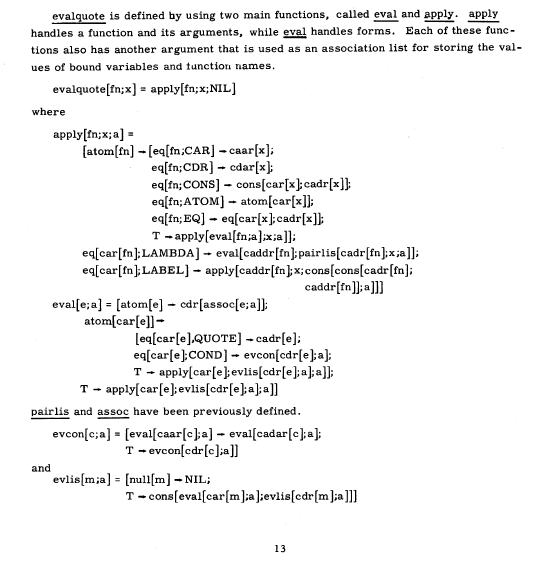
\includegraphics{Lisp_Maxwells_Equations}
\caption{McCarthy's Equations of Software}
\end{figure}
\input{Lisp}

\end{document}